\section{Additional Analysis}
\label{app:analysis}

\subsection{Store Size and Filter Characterization}

Across methods a larger store does not buy a higher pass rate
(Section~\ref{sec:exp1}). Within a fixed method the same growth can instead
represent useful signal. Across models, richer feedback grows the store from
200 to 235 KB with \cond{Self-Judge} to 328 to 343 KB with
\cond{Checkpoint-binary + Human} while improving checkpoint pass rate
(Table~\ref{tab:exp2-full}). Under rich feedback, repeated rounds grow the
store from 328 to 343 KB at R1 to 575 to 603 KB at R4 while
performance continues to improve (Table~\ref{tab:exp4-rich}). These within-method results distinguish the Filter Hypothesis from
a simple compression objective.

\subsection{Rollout-Volume Control}

This control asks whether the R4 result follows from the number of
rollouts consolidated. Pooled \cond{Insights} and \cond{No Consolidation} each
receive 635 rollouts from R0 to R4, more than the 508 the evaluated
\cond{Free Form} R4 store was built from, and consolidate them in a single pass
rather than one batch at a time. On strictly more rollouts, pooled
\cond{Insights} only reaches about what \cond{Free Form} reached from the 254
rollouts behind its R2 store, and it remains 6.1 to 7.1 pp below
\cond{Free Form} R4 for every model
(Figure~\ref{fig:rollout-volume-control}). Rollout volume therefore does not
account for the R4 result. Because the pooled runs also change the consolidation
method, this control rules volume out as the explanation without establishing
incremental consolidation as the cause.

\begin{figure}[h]
\centering
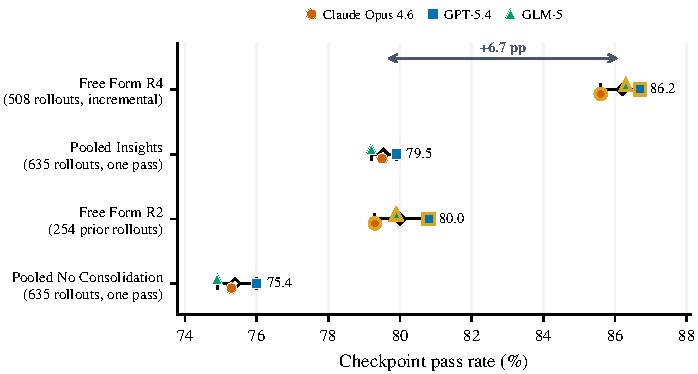
\includegraphics[width=0.78\linewidth]{fig_experience_volume_control.pdf}
\caption{\textbf{Rollout volume does not account for the R4 result.}
Colored markers show individual model variants. Black diamonds and
whiskers show the cross-model mean and min to max range.
The pooled controls consume 635 rollouts from R0 to R4, more than the
508 the \cond{Free Form} R4 store was built from, and consolidate them in one
pass while \cond{Free Form} consolidates one batch at a time.
Exact results appear in Table~\ref{tab:pooled-full}.}
\label{fig:rollout-volume-control}
\end{figure}

\subsection{Task-Score Distributions}

\begin{figure}[h]
\centering
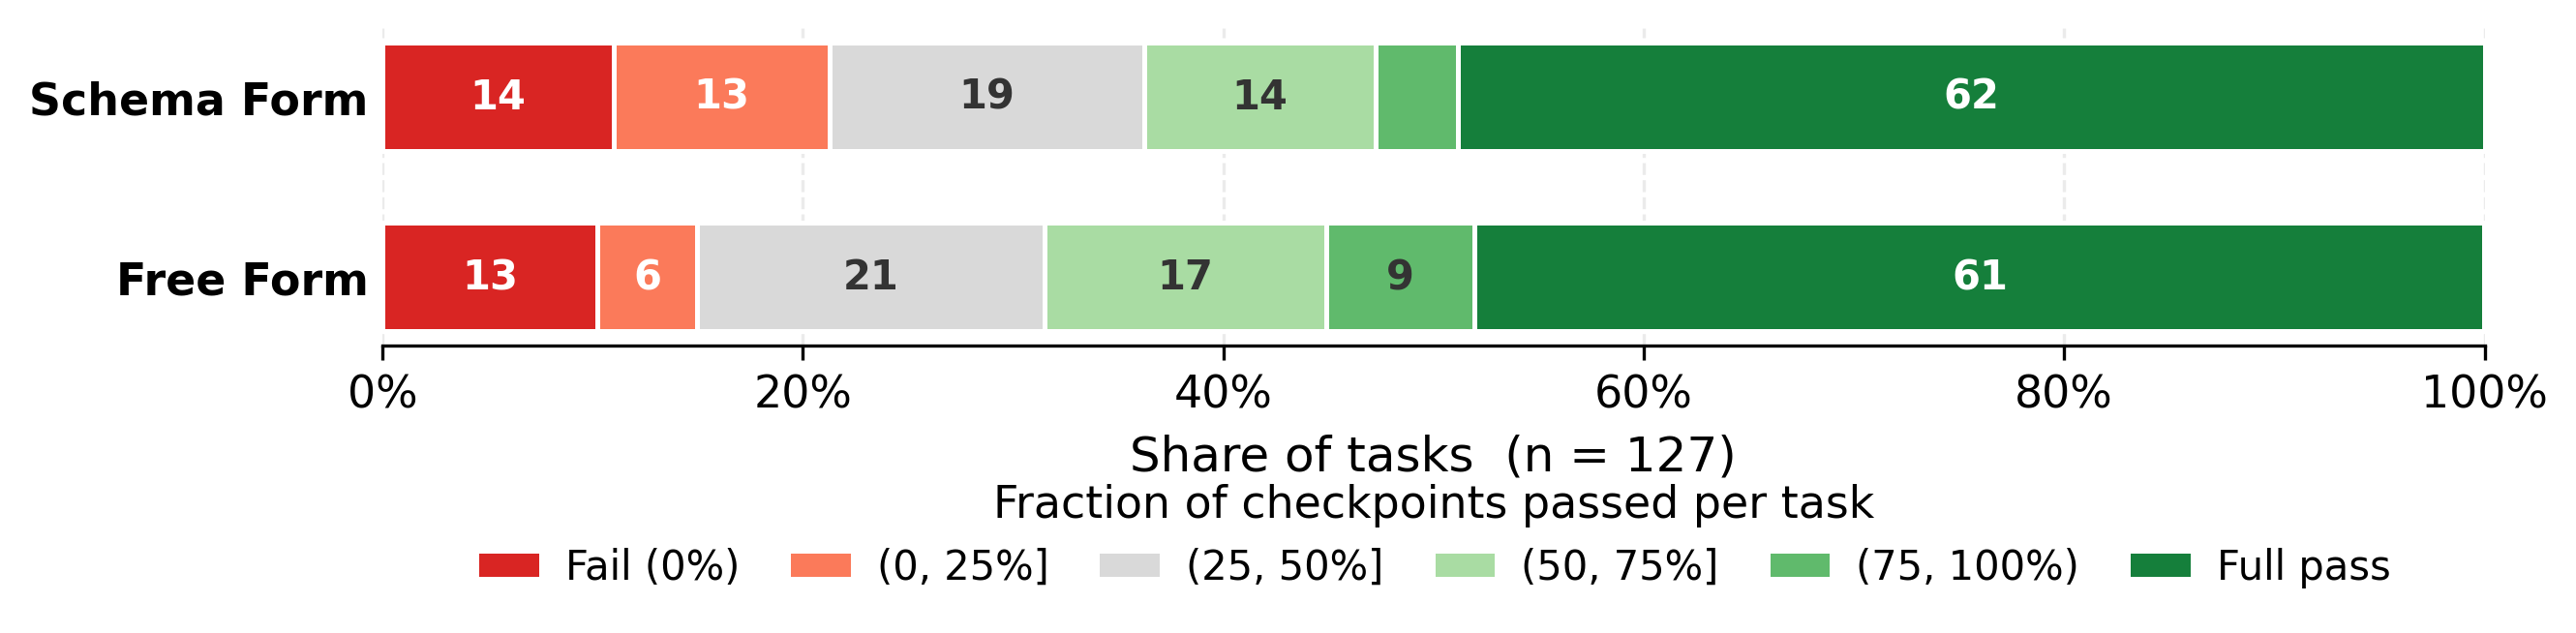
\includegraphics[width=0.88\linewidth]{exp1_schema_vs_free_buckets.png}
\caption{\textbf{\cond{Free Form} versus \cond{Schema Form} by task-score bucket for Claude
Opus 4.6.} The checkpoint-level advantage of \cond{Free Form} is distributed across
partially completed tasks, while \cond{Schema Form} narrowly leads in the
all-or-nothing fully-passed rate. This difference motivates reporting both
metrics.}
\label{fig:schema-free-distribution}
\end{figure}

\subsection{Failure-Cause Statistics and Analysis}

\subsection{Task-Score Bucket Counts}

\subsection{Selection of the Qualitative Examples}

\subsection{Qualitative Consolidation Behaviors}

\begin{table}[h]
\caption{\textbf{Representative filtering behaviors observed in generated
stores.} These examples motivate, rather than independently prove, the Filter
Hypothesis.}
\label{tab:qualitative-filter}
\centering
\small
\begin{tabularx}{\linewidth}{@{}lXX@{}}
\toprule
Behavior & Observed pattern & Procedural consequence \\
\midrule
Implicit merge &
Free Form revises one GitLab authentication wiki page with new pagination and error
handling evidence. &
Repeated trials become one richer procedure. \\
Independent duplication &
SkillX creates 15 separate pages describing substantially the same GitLab API
authentication procedure. &
Retrieval must sift through redundant fragments. \\
Schema omission &
On \texttt{ds-stock-analysis-slides}, Schema Form records step names but drops
the code and formatting details retained by Free Form. &
The action is named but not reliably executable. \\
Explicit false merge &
Schema Form-ED merges ``grade ML exams with Python'' and ``extract video frames
with Python'' under \texttt{action-bash-run-python}. &
Unrelated instructions can be retrieved together. \\
\bottomrule
\end{tabularx}
\end{table}
